\section{Partial Differential Equations}

\renewcommand{\arraystretch}{1.3}
\begin{tabularx}{0.98\linewidth}{@{}lllclp{0.28\linewidth}@{}}
    \toprule
            & \multicolumn{2}{c}{1D} & \phantom{.}            & \multicolumn{2}{c}{2D}                                                                                                                         \\ %chktex 2
    \cmidrule{2-3} \cmidrule{5-6}
            & finite                 & infinite               &                        & rectangle                    & disc                                                                                   \\%chktex 2
    \cmidrule{1-6}
    Wave    & \ref{ssec:1d_wave_FS}  & \ref{ssec:1d_wave_Al}  &                        & \ref{ssec:2d_wave_rect}                                                                                               \\%chktex 2
    Heat    & \ref{ssec:1d_heat_fin} & \ref{ssec:1d_heat_inf} &                        &                                                                                                                       \\%chktex 2
    Laplace &                        &                        &                        & \ref{sssec:laplace_dir_rect} & Dirichlet:~\ref{sssec:laplace_dir_radial}\newline Neumann:~\ref{sssec:laplace_neu_rad} \\%chktex 2
    \bottomrule
\end{tabularx}
\renewcommand{\arraystretch}{1}


\subsection{Definition}
A partial differential equation (PDE) is an equation involving an \textbf{unknown function} (in contrast to ODEs only one) and some of its \textbf{partial derivatives}.
\begin{enumerate}
    \item A PDE is called \textbf{linear} if it is linear in the unknown function u and its derivatives.
    \item A linear PDE is called \textbf{homogeneous} if each of its terms contains either the function or one of its derivatives.
    \item The \textbf{order} of a PDE is the order of the highest derivative in the PDE.\@
\end{enumerate}

\subsubsection{Basic Types of PDEs}
\begin{itemize}
    \item 1-dimensional Wave Equation:
          \begin{equation*}
              \frac{\partial ^2 u}{\partial t^2} = c^2\frac{\partial u}{\partial x^2}
          \end{equation*}
          (\textit{linear, 2nd order, homogeneous, hyperbolic})
    \item 1-dimensional Heat Equation:
          \begin{equation*}
              \frac{\partial u}{\partial t} = c^2 \frac{\partial ^2 u}{\partial x^2}
          \end{equation*}
          (\textit{linear, 2nd order, homogeneous, parabolic})
    \item 2-dimensional Laplace Equation:
          \begin{equation*}
              \nabla^2 u=\frac{\partial^2 u}{\partial x^2}+\frac{\partial ^2 u}{\partial y^2}=0
          \end{equation*}
          (\textit{linear, 2nd order, homogeneous, elliptic})
    \item 2-dimensional Poisson Equation:
          \begin{equation*}
              \nabla^2 u=\frac{\partial^2 u}{\partial x^2}+\frac{\partial^2 u}{\partial y^2}=f(x,y)
          \end{equation*}
          (\textit{linear, 2nd order, inhomogeneous, elliptic})
    \item 2-dimensional Wave Equation:
          \begin{equation*}
              \frac{\partial^2u}{\partial t^2}=c^2 \Bigl(\frac{\partial^2 u}{\partial x^2}+\frac{\partial ^2 u}{\partial y^2}\Bigr)=c^2\nabla^2 u
          \end{equation*}
          (\textit{linear, 2nd order, homogeneous, hyperbolic})
    \item 2-dimensional Heat Equation
          \begin{equation*}
              \frac{\partial u}{\partial t}=c^2\Bigl(\frac{\partial^2 u}{\partial x^2}+\frac{\partial ^2 u}{\partial y^2}\Bigr)=c^2\nabla^2 u
          \end{equation*}
          (\textit{linear, 2nd order, homogeneous, parabolic})
    \item 3-dimensional Laplace Equation
          \begin{equation*}
              \nabla^2 u=\frac{\partial^2 u}{\partial x^2}+\frac{\partial ^2 u}{\partial y^2}+\frac{\partial ^2 u}{\partial z^2}=0
          \end{equation*}
          (\textit{linear, 2nd order, homogeneous, elliptic})
\end{itemize}

\subsubsection{Solutions of linear PDEs}
\begin{itemize}
    \item Many functions of a certain form can satisfy the PDE
    \item Uniqueness of solutions is achieved by \textbf{boundary} conditions and \textbf{initial} conditions
\end{itemize}
\vspace{5pt}
\textbf{Superposition Principle}\\
If $u_{1}$ and $u_{2}$ are solutions of a \textbf{homogeneous} (linearity is not enough) PDE, then $\alpha u_{1} + \beta u_{2}$ is also a solution of the same PDE $\forall \alpha , \beta \in \mathbb{R}$

\subsection{2nd Order Linear PDEs}
\subsubsection{General Form of 2nd Order Linear PDE}
A 2nd order linear PDE can be written in the form
\begin{equation*}
    Au_{xx}+2Bu_{xy}+Cu_{yy}=F(x,y,u,u_x,u_y)
\end{equation*}

\subsubsection{Classification by Discriminant}
A 2nd order linear PDE has the discriminant $AC-B^2$ and is called
\begin{enumerate}
    \item \textbf{hyperbolic} (wave), if $AC-B^2<0$
    \item \textbf{parabolic} (heat), if $AC-B^2=0$
    \item \textbf{elliptic} (laplace), if $AC-B^2>0$
\end{enumerate}
\vspace{5pt}
Remarks:
\begin{itemize}
    \item Classification is independent of the PDEs dimension\vspace{5pt}
    \item The type of a PDE depends only on the terms of second order: \textbf{Poisson} equations are also \textbf{elliptic}.
\end{itemize}

\subsection{1D Wave Equation - Fourier Series}\label{ssec:1d_wave_FS}
To find $u(x,t)$ satisfying the \textbf{homogeneous} 1D wave equation on $x\in[0,L]$ with \textbf{initial} and
\textbf{boundary} conditions:
\begin{equation*}
    \begin{cases}
        u_{tt}=c^2u_{xx} & \text{PDE} \\
        u(0,t)=u_0       & \text{BC}  \\
        u(L,t)=u_L       & \text{BC}  \\
        u(x,0)=f(x)      & \text{IC}  \\
        u_t(x,0)=g(x)    & \text{IC}
    \end{cases}
\end{equation*}\\
three steps have to be taken:
\begin{itemize}
    \item[(i)] Separation of variables
    \item[(ii)] Finding the ``many'' solution
    \item[(iii)] Finding one solution satisfying IC \& BC
\end{itemize}

\subsubsection{(i) Separation of Variables}
\begin{align*}
    u(x,t)                          & =F(x)G(t)                                               \\
    \underbrace{F\ddot{G}}_{u_{tt}} & =c^2\underbrace{F''G}_{u_{xx}}                          \\
    \frac{\ddot{G}}{c^2G}           & =\frac{F''}{F}=k\hspace*{10pt}\Rightarrow\hspace*{10pt}
    \begin{cases}
        F''=kF \\
        \ddot{G}=c^2kG
    \end{cases}
\end{align*}
\begin{align*}
    u(0,t) & =F(0)G(t)=u_0\mathrm{~}\forall t\geq0\quad\Rightarrow & \mathbf{F(0)}=\mathbf{u_0} \\
    u(L,t) & =F(L)G(t)=u_L\mathrm{~}\forall t\geq0\quad\Rightarrow & \mathbf{F(L)}=\mathbf{u_L}
\end{align*}

\subsubsection{(ii) ``Many'' Solution}
By applying the boundary conditions \textbf{BC}
\begin{align*}
    \mathbf{F(0)} & =\mathbf{u_0} \\
    \mathbf{F(L)} & =\mathbf{u_L}
\end{align*}
into the separated equation
\begin{equation*}
    F''=kF \\
\end{equation*}
$F(x)$ can be found:
\begin{align*}
    F(x)= &
    \begin{cases}
        A_1e^{\sqrt{k}x}+A_2e^{-\sqrt{k}x}      & k>0 \\
        A_1\cos(\sqrt{-k}x)+A_2\sin(\sqrt{-k}x) & k<0 \\
        A_1x+A_2                                & k=0 \\
    \end{cases} \\
\end{align*}
Since $k$ is constant for both $F,G$, $G(t)$ satisfying
\begin{align*}
    \ddot{G}=c^2kG
\end{align*}
can be obtained by:
\begin{align*}
    G(t)= &
    \begin{cases}
        B_1e^{\sqrt{k}t}+B_2e^{-\sqrt{k}t}      & \;\,k>0 \\
        B_1\cos(\sqrt{-k}t)+B_2\sin(\sqrt{-k}t) & \;\,k<0 \\
        B_1t+B_2                                & \;\,k=0
    \end{cases}
\end{align*}
The ``Many'' Solution are the linear combination of all possible $F(x)$ and $G(t)$.
\begin{equation*}
    u(x, t) = \sum_{n=1}^{\infty}u_n(x,t) = \sum_{n=1}^{\infty}F_n(x)G_n(t)
\end{equation*}

\subsubsection{(iii) Specific Solution}\label{pde/1dwave/specificSolution}
In general, the specific solution can be found by combining the initial conditions \textbf{IC}
with the general solution found in (ii).\\\hbox{}\\
If $\mathbf{u(0,t)=u(L,t)= 0}$ the \textbf{general solution} Ansatz:
\begin{equation*}
    u(x,t)=\sum\limits_{n=1}^{\infty}
    \Bigl( B_n \cos(\lambda _n t)+B_n^* \sin(\lambda_n t)\Bigr) \sin
    \left(\frac{n \pi}{L}x \right)
\end{equation*}\\
can be used, and the \textbf{specific solution} by \textbf{FS} is given by:
\begin{align*}
    \lambda_n & =\frac{c\; n\; \pi}{L}                                               \\
    B_n       & =\frac{2}{L}\int\limits_0^L f(x)\sin(\frac{n\;\pi}{L}x)dx            \\
    B_n^*     & =\frac{2}{L\lambda_n} \int\limits_0^L g(x) \sin(\frac{n\;\pi}{L}x)dx \\\\
    f(x)      & =\sum\limits_{n=1}^{\infty} B_n \sin(\frac{n\;\pi}{L}x)              \\
    g(x)      & =\sum\limits_{n=1}^{\infty} B_n^* \lambda_n \sin(\frac{n\;\pi}{L}x)  \\
\end{align*}
\text{Useful tricks:}
\begin{itemize}
    \item If $f(x),g(x)$ can be written in terms of $\sin(\frac{n\;\pi}{L}x)$, $B_n, B_n^*$
          can be calculated directly
\end{itemize}

\subsubsection{Inhomogeneous Boundary Conditions}
To solve a linear homogeneous 2nd order PDE with inhomogeneous BC, a fitting substitution can be used:
\begin{align*}
     & v(x,t):= u(x,t) -w(x) \\
     & \begin{cases}
           v_{tt}=c^2v_{xx}     \\
           v(0,t)=u(0,t)-w(0)=0 \\
           v(L,t)=u(L,t)-w(L)=0 \\
           v(x,0)=u(x,0)-w(x)   \\
           v_t(x,0)=u_t(x,0)
       \end{cases}
\end{align*}
subsequently, $v(x,t)$ has homogeneous BC.

\begin{examplesection}[Example]
    For the given Problem
    \[ u_{tt}=c^2u_{xx}\]
    we make the Ansatz
    \[u(x,t)=F(x)G(t)\]
    Plugging this into the given PDE and rearranging delivers
    \[u_{tt}=F\ddot{G};\qquad u_{xx}=F''G \quad \rightarrow F\ddot{G}=c^2F''G\]
    \[\frac{\ddot{G}}{c^2G}=\frac{F''}{F}=k\;\; ;\qquad\quad\begin{cases} F''=kF \\
            \ddot{G}=c^2kG
        \end{cases}\]
    as $k$ must be constant. This rearrangement is the purpose of our Ansatz and delivers two ODEs to solve instead of one PDE.
    Inserting the boundary conditions into $F''=kF$ and using a harmonic Ansatz delivers a set of solutions for the BVP of the form
    \[F_n (x)=\sin{\left( \frac{n \pi}{L} x \right) }, \sqrt{-k}=\frac{n \pi}{L}\]
    which satisfy the BVP for negative values of k ($k \ge 0$ yields the $F=0$ solution which is not interesting).\\
    Inserting these values of $k$ into $\ddot{G}=c^2kG$ and using a harmonic Ansatz again delivers a family of solutions
    \[G_n (t) =  B_n \cos{(\lambda_{n} t)} + B_n^* \sin{(\lambda_{n}t)}\]
    where
    \[ \lambda_{n} = \frac{c n \pi}{L} \]
    Inserting $F_n$ and $G_n$ into $u(x,t)=F(x)G(t)$ we obtain a family of solutions for our initial problem of the form
    \[u_n (x, t) = (B_n \cos{(\lambda_{n} t)} + B_n^* \sin{(\lambda_{n}t)})\sin{\left( \frac{n \pi}{L} x \right) } \]
    where $u_n (x, t)$ are called Eigenfunctions and $\lambda_n$ the spectrum.\\
    Using fourier series we can generate a general solution for all $n$ of the form
    \[u(x,t)=\sum\limits_{n=1}^{\infty}\begin{pmatrix}
            B_n \cos(\lambda _n t)+B_n^* \sin(\lambda_n t)
        \end{pmatrix} \sin\left(\frac{n \pi}{L}x \right) \]
    which does not satisfy the IVP in general.\\
    To satisfy the IVP we insert the initial value conditions $u(x,0)=f(x)$ and $u_t(x,0)=g(x)$ from which we obtain the formulas shown in Chapter~\ref{pde/1dwave/specificSolution}.
\end{examplesection}

\subsection{1D Wave Equation - d'Alembert}\label{ssec:1d_wave_Al}
The \textit{D'Alembert} solution $u(x,t) = \phi(x+ct)+\psi(x-ct)$ is the general solution to the 1D wave equation IVP.
\begin{equation*}
    \begin{cases}
        u_{tt} = c^2u_{xx} & x \in \mathbb{R}, t \geq 0 \\
        u(x,0) = f(x)      & x \in \mathbb{R}           \\
        u_t(x,0) = g(x)    & x \in \mathbb{R}
    \end{cases}
\end{equation*}
the \textit{D'Alembert} solution can be rewritten as following:
\begin{equation*}
    u(x,t)=\frac{1}{2}\left[f(x+ct)+f(x-ct)\right]+\frac{1}{2c}\int_{x-ct}^{x+ct}g(s)ds
\end{equation*}
This form shows, that for a given position $x_i$ and time $t_i$ the result is only depending on the initial position \textcolor{mathGreen}{$f(\cdot)$} at \textcolor{mathGreen}{$x_i\pm ct_i$} and the initial velocity \textcolor{red}{$g(\cdot)$} evaluated over the interval \textcolor{red}{$x_i\pm ct_i$}.
\begin{center}
    \begin{tikzpicture}
        \begin{axis}[
                width=0.8\linewidth,
                unit vector ratio={1 1},
                axis x line=left,
                axis y line=left,
                xmin=0,
                xmax=4,
                ymin=0,
                ymax=1.5,
                xlabel={$x$},
                ylabel={$t$},
                xtick={1,3},
                xticklabels={\textcolor{blue}{$x_i-ct_i$}, \textcolor{blue}{$x_i-ct_i$}},
                ytick={0},
                mark=none,
            ]
            \addplot [blue]
            coordinates {
                    (1,0)
                    (2,1)
                };
            \addplot [blue]
            coordinates {
                    (3,0)
                    (2,1)
                };
            \addplot [red, very thick]
            coordinates {
                    (1,0.01)
                    (3,0.01)
                };
            \addplot[color=mathGreen, fill=mathGreen, only marks,mark=*]
            coordinates{
                    (1,0)
                    (3,0)};
            \node[label={[right,yshift=1ex,xshift=0.3em]:{\textcolor{blue}{($x_i,t_i$)}}},circle,fill=white,draw=blue, thick, inner sep=1pt]
            at (axis cs:2,1) {};
        \end{axis}
    \end{tikzpicture}
\end{center}
If the initial conditions $f(\cdot)$ and $g(\cdot)$ are only non zero on the interval $[a,b]$ the solution of the wave equation can be divided into the following six sectors ($I-VI$).
\includegraphics[width=\linewidth]{../images/pde_dAlembert.png}
where $u(x_i,t_i)$ is
\begin{equation*}
    \begin{cases}
        0,                                                                        & \forall (x_i,t_i) \in I \cup III \\
        \text{full d'Alembert equation}                                           & \forall (x_i,t_i) \in II         \\
        \frac{1}{2c}\int_{a}^{b}g(s)ds                                            & \forall (x_i,t_i) \in V          \\
        \frac{1}{2}\left[f(x_i+ct_i)\right]+\frac{1}{2c}\int_{a}^{x_i+ct_i}g(s)ds & \forall (x_i,t_i) \in IV         \\
        \frac{1}{2}\left[f(x_i-ct_i)\right]+\frac{1}{2c}\int_{x_i-ct_i}^{b}g(s)ds & \forall (x_i,t_i) \in VI
    \end{cases}
\end{equation*}


\subsection{Normal Form}
With an appropriate change of coordinates a 2nd order linear PDE can be brought into the \textit{normal form}, that is
\begin{align*}
    u_{vw}=F^{*}(v,w,u,u_{v},u_{w})        &  & \text{if hyperbolic} \\
    u_{vv}=F^{*}(v,w,u,u_{v},u_{w})        &  & \text{if parabolic}  \\
    u_{vv}+u_{ww}=F^{*}(v,w,u,u_{v},u_{w}) &  & \text{if elliptic}
\end{align*}

\subsubsection{Substitutions}
\begin{align*}
    v=\varphi(x,y)\quad\text{and}\quad w=\psi(x,y)                   &   & \text{if hyperbolic} \\
    v=x\quad\text{and}\quad w=\psi(x,y)                              &   & \text{if parabolic}  \\
    v=\frac{1}{2}\Bigl(\varphi(x,y)+\psi(x,y)\Bigr)                  &   & \text{if elliptic}   \\
    \text{and}\quad w=\frac{1}{2i}\Bigl(\varphi(x,y)-\psi(x,y)\Bigr) &
\end{align*}

\subsubsection{Steps}
\begin{enumerate}
    \item Check if PDE is hyperbolic, parabolic or elliptic:
          \begin{align*}
              A(x,y)u_{xx}+2B(x,y)u_{xy} & +C(x,y)u_{yy}          \\
                                         & =F(u,u_x,u_y,x,y)      \\\\
              B(x,y)-A(x,y)C(x,y)        & \begin{cases}
                                               >0 & \text{hyperbolic} \\
                                               =0 & \text{parabolic}  \\
                                               <0 & \text{elliptic}
                                           \end{cases}
          \end{align*}
    \item Formulate the characteristic equation:
          \begin{align*}
              A(x,y){(y')}^2-2B(x,y)y'+C(x,y)\overset{!}{=} 0
          \end{align*}
    \item Obtain $C_{1},C_{2}$ by solving the characteristic equation by setting
          \begin{align*}
              y'=\frac{\partial\, y}{\partial x}
          \end{align*}
    \item Perform change of variables:
          \begin{align*}
              v = C_{1} \quad w=C_{2}
          \end{align*}
    \item Calculate $v_{x},v_{y},w_{x},w_{y}$
          and write $u_{x},u_{xx},u_{yx},u_{yy},F$ in terms of
          $u_{v},u_{w},u_{vw},u_{vv},u_{ww}$ if applicable.
    \item Obtain the \textit{normal form} $u_{v,w}$
    \item Obtain $u(x,y)$ by integrating the \textit{normal form} $u(v,w)$
          and re-substitution:
          \begin{align*}
              u(v,w) & =\iint u_{wv}\ dwdv         \\
              u(x,y) & =u(v,w)|_{v=C_{1}, w=C_{2}}
          \end{align*}
\end{enumerate}

\subsection{1D Heat Equation - Finite Domain}\label{ssec:1d_heat_fin}
\subsubsection{Boundary Condition \texorpdfstring{$u(0,t), u(L,t)$}{u (0,t), u (L,t)}}
The PDE $u_t=c^2u_{xx}$ with boundary conditions $u(0,t)=u(L,t)=0$, $u(x,0)=f(x)$
and $x\in[0,L]$ can be solved with the \textbf{Fourier Series Ansatz} resulting
from separation of variables:
\begin{align*}
    u(x,t) & =\sum_{n=1}^\infty B_n\sin(\frac{n\pi}Lx)e^{-\lambda_n^2t}                                \\
    B_n    & =\dfrac{2}{L}\int\limits_0^{L}f(x)\sin(\dfrac{n\pi}{L}x)dx & \lambda_n, = \frac{cn\pi}{L}
\end{align*}

\subsubsection{Boundary Condition \texorpdfstring{$u_{t}(0,t),u_{t}(L,t)$}{ut (0,t), ut (L,t)}}
The PDE $u_{t}=c^2u_{xx}$ with boundary conditions $u_t(0,t)=u(L,t)=0$, $u_t(x,0)=f(x)$
and $x\in[0,L]$ can be solved by \textbf{separation of variables}:
\begin{enumerate}
    \item $u(x,t)=F(x)G(t)$
    \item find $F(x),G(t)$ by inserting the boundary conditions $u_t$
    \item use superposition:
          \begin{equation*}
              u(x,t)=\sum_{n=0}^{\infty} \underbrace{F_n(x)G_n(t)}_{u_n(x,t)}
          \end{equation*}
    \item use additional boundary conditions to find the coefficients for $u(x,t)$
\end{enumerate}
{\color{gray}\hrule}\, \\
Alternatively, if $f(x)$ can be written as (e.g.\@ by setting $t = 0$)
\begin{equation*}
    u(x,t)=\sum_{n=0}^{\infty}a_n\cos(nx)e^{-c^2n^2t}
\end{equation*}
this general Ansatz can be used.
\subsubsection{Time Dependent Heat Equation}
If the heat equation is time dependent, for example if
\begin{equation*}
    u(x,t)=
    \begin{cases}u_t=2tc^2u_{xx} & x\in[0,L],t\in[0,+\infty) \\% chktex 9
             u(0,t)=0        & t\in[0,+\infty)           \\% chktex 9
             0               & t\in[0,+\infty),          % chktex 9
    \end{cases}
\end{equation*}
the separation of variables results in
\begin{equation*}
    \begin{cases}
        F''     & =kF      \\
        \dot{G} & =2kc^2tG
    \end{cases}
\end{equation*}
and therefore the \textbf{Fourier Series Ansatz} only differs in $G_n(t)$.
In this example, this results in
\begin{equation*}
    u(x,t) =\sum_{n=1}^\infty B_n\sin(\frac{n\pi}Lx)e^{-\lambda_n^2t^2}.
\end{equation*}

\subsection{1D Heat Equation - Infinite Domain}\label{ssec:1d_heat_inf}
The heat equation on an infinite domain
\begin{equation*}
    \begin{cases}
        u_t=c^2u_{xx} & x\in \mathbb{R} \\
        u(x,0)=f(x)   & x\in \mathbb{R}
    \end{cases}
\end{equation*}
can either be solved by using the \textbf{Fourier Integral} or \textbf{Fourier Transform}.
In both cases, the solution can be found by:
\begin{equation*}
    u(x,t)=\frac{1}{2c\sqrt{\pi t}}\int_{-\infty}^{\infty}f(v)\exp\left[-{\left(\frac{x-v}{2c\sqrt{t}}\right)}^{2}\right]dv
\end{equation*}


\subsubsection{Fourier Integral}
Separation of variables results in the following the Fourier integral:
\begin{align*}
    u(x,t) & =\int_0^\infty(A(p)\cos(px)+B(p)\sin(px))e^{-c^2p^2t}dp \\
    A(p)   & =\frac1\pi\int_{-\infty}^\infty f(v)\cos(pv)dv          \\
    B(p)   & =\frac1\pi\int_{-\infty}^\infty f(v)\sin(pv)dv
\end{align*}
\textbf{Hint!} $A(p)=0$ if $f(x)$ is odd and $B(p)=0$ if $f(x)$ is even.


\subsubsection{Fourier Transform}
\begin{enumerate}
    \item By applying the \textbf{Fourier transform} with respect to $x$, the PDE can be
          transformed into an ODE:
          \begin{align*}
              \mathcal{F}_x\Bigl\{u_t(x,t)\Bigr\} & =\mathcal{F}_x\Bigl\{c^2u_{xx}(x,t)\Bigr\} \\
              \hat{u}_t(w,t)                      & =-c^2w^2\hat{u}(w,t)
          \end{align*}
    \item Transform the initial conditions with respect to $x$. (Explicit calculation maybe not needed!)
          \begin{equation*}
              \widehat{f}(w)=\mathcal{F}_x\Bigl\{f(x)\Bigr\}
          \end{equation*}
    \item Solve the ODE with initial conditions
          \begin{align*}
              \hat{u}(w,t) & =C(w)e^{-c^2w^2t}                             \\
              \hat{u}(w,0) & =\hat{f}(w)\;\Leftrightarrow\;\hat{f}(w)=C(w) \\
              \hat{u}(w,t) & =\hat{f}(w)e^{-c^2w^2t}
          \end{align*}
    \item Obtain final solution by inverse FT (Check~\ref{known_transforms}):
          \begin{equation*}
              u(x,t)=\mathcal{F}_x^{-1}\Bigl\{\widehat{u}(w,t)\Bigr\}
          \end{equation*}
\end{enumerate}
\textbf{Remark} This approach is not exclusive to the heat equation on an infinite domain, but can be used
on any PDE.

\subsection{Laplace Equation}\label{ssec:laplace}
The steady-state solution of the 2-dimensional heat equation can be reduced to the Laplace equation $\nabla^2 u=0$, where $\nabla^2$ is the \textit{Laplacian operator}. Functions that satisfy the Laplace equation are called \textit{harmonic}. \\
Depending on the boundary conditions on the region $R$ three distinct cases exist:
\begin{itemize}
    \item \textbf{Dirichlet BC}: For the \textit{Dirichlet problem} $u$ is prescribed on the boundary $\partial R$ of $R$;
    \item \textbf{Neumann BC}: For the \textit{Neumann problem} the normal partial derivative $u_n$ is prescribed on $\partial R$;
    \item \textbf{Robin BC}: The \textit{Robin problem} is a combination of both aforementioned.
\end{itemize}

\subsubsection{2D Dirichlet Problem on a Rectangle}\label{sssec:laplace_dir_rect}
The two-dimensional steady-state solution with \textit{Dirichlet BC} on a rectangle $R$
\begin{equation*}
    \begin{cases}
        \nabla^2 u=0 & R = \{(x,y) : x\in [0,a], y\in [0,b]\} \\
        u(0,y)=0                                              \\
        u(a,y)=0                                              \\
        u(x,0)=0                                              \\
        u(x,b)=f(x)
    \end{cases}
\end{equation*}
can be solved with the \textbf{Fourier Series Ansatz} obtained from separation of variables:
\begin{align*}
    u(x,y)=\sum_{n=1}^{\infty}A_{n}\sin(\frac{n\pi}ax)\sinh(\frac{n\pi}ay) \\
    A_{n}=\frac{2}{a\sinh(\frac{n\pi}{a}b)}\int^{a}f(x)\sin(\frac{n\pi}{a}x)dx
\end{align*}
\textbf{Hints:} If the prescribed boundary condition is given on an edge other than $u(x,b)$, a variable transform is necessary. If more than one boundary has a prescribed function $\widetilde{f}\neq0$, the
individual solutions for each boundary can be superpositioned. (See Appendix~\ref{diri_superpos})

\subsubsection{2D Dirichlet Problem with Radial Symmetry}\label{sssec:laplace_dir_radial}
For a Laplace equation on a disk $D$ with radius $R$
\begin{equation*}
    \begin{cases}
        \nabla^2 u=0, & D=\{(x,y): x^2+y^2 < R^2\}          \\
        u(x,y)=f      & \partial D=\{(x,y): x^2+y^2 = R^2\} \\
    \end{cases}
\end{equation*}
the solution to the Dirichlet problem given by
\begin{equation*}
    u(r,\theta)=\sum_{n=0}^\infty r^n(A_n\cos(n\theta)+B_n\sin(n\theta))
\end{equation*}
with
\begin{align*}
     & A_{0} =\frac{1}{2\pi}\int_0^{2\pi}f(\varphi)d\varphi                 \\
     & A_{n} =\frac{1}{R^n\pi}\int_0^{2\pi}f(\varphi)\cos(n\varphi)d\varphi \\
     & B_{n} =\frac{1}{R^n\pi}\int_0^{2\pi}f(\varphi)\sin(n\varphi)d\varphi
\end{align*}
This can be further simplified to the \textit{Poisson integral form}
\begin{equation*}
    u(r,\theta)=\frac{1}{2\pi}\int_0^{2\pi}K(r,\theta,R,\varphi)f(\varphi)d\varphi
\end{equation*}
where $K(r,\theta,R,\varphi)$ is the \textit{Poisson integral kernel}
\begin{equation*}
    K(r,\theta,R,\varphi):=\frac{R^2-r^2}{R^2-2rR\cos(\theta-\varphi)+r^2}.
\end{equation*}

\textbf{Remark}
To get to the given equation the following coordinate transform was applied:
\begin{equation*}
    \begin{cases}
        x=r\cos\theta \\
        y=r\sin\theta
    \end{cases}
    \:\Leftrightarrow\:
    \begin{cases}
        r={(x^2+y^2)}^{1/2} \\
        \theta=\arctan\frac yx.
    \end{cases}
\end{equation*}
Which results in Laplace equation
\begin{equation*}
    \begin{cases}
        u_{rr} + \frac{1}{r^2}u_{\theta\theta}+\frac{1}{r}u_r = 0 & \text{on } D          \\
        u(R,\theta)=f(\theta)                                     & \text{on } \partial D
    \end{cases}
\end{equation*}
\textbf{Hint!} If $u(R,\theta)=f(\theta)$ itself fulfils the Laplace equation $\nabla^2u=0$, its the solution
to the \textit{2D Dirichlet problem with radial symmetry}

\subsubsection{2D Neumann Problem with Radial Symmetry}\label{sssec:laplace_neu_rad}
Similar to the \textit{2D Dirichlet problem with radial symmetry} (\ref{sssec:laplace_dir_radial})
the solution of the 2D Neumann problem with radial symmetry on a disk $D$
\begin{equation*}
    \begin{cases}
        u_{rr} + \frac{1}{r^2}u_{\theta\theta}+\frac{1}{r}u_r = 0 & \text{on } D          \\
        u_r(R,\theta)=f(\theta)                                   & \text{on } \partial D
    \end{cases}
\end{equation*}
is given by
\begin{equation*}
    u(r,\theta)=A_0+\sum_{n=1}^\infty r^n(A_n\cos(n\theta)+B_n\sin(n\theta))
\end{equation*}
with
\begin{align*}
    A_n & =\frac{1}{nR^{n-1}\pi}\int_{0}^{2\pi}f(\xi)\cos(n\xi)d\xi \\
    B_n & =\frac{1}{nR^{n-1}\pi}\int_{0}^{2\pi}f(\xi)\sin(n\xi)d\xi \\
    A_0 & = \text{undefined constant}
\end{align*}

\textbf{Checking if a Solution Exists}\\
A solution of the \textit{2D Laplace equation with Neumann borders}
\begin{align*}
    \begin{cases}
        \nabla^2u=f                       & \text{in } R          \\
        \frac{\partial u}{\partial n} = g & \text{on } \partial R
    \end{cases}
\end{align*}
only exists if
\begin{equation*}
    \int_R f \;dA = \int_{\partial R} g \;dx
\end{equation*}
due to the Gauss/ divergence theorem (2D):
\begin{align*}
    \int_{\partial R} \underbrace{\frac{\partial u}{\partial n}}_{g}  \; dx
    =\int_{\partial R} \nabla u\cdot\vec{n}\; dx \overset{\text{Gauss}}{=} & \int_R \underbrace{\text{div}(\nabla u)}_{\nabla^2 u=f}\; dA
\end{align*}

\subsubsection{Maximum Principle}
Functions that satisfy the Laplace equation $\nabla^2 u=0$ are called \textit{harmonic} functions. A harmonic function is equal at any point to the average of the values on \textit{any} circle centered at that point, hence
\begin{equation*}
    u(x_0, y_0)=\frac{1}{2\pi}\int_{0}^{2\pi}u(a,\varphi)d\varphi
\end{equation*}
\includegraphics*[width=\linewidth]{pde_harmonic_function.png}

\textbf{Maximum principle}

The above property demands: If a harmonic function $u$ takes its maximum values on the interior of the region $D$ where it is harmonic, then it must be \textbf{constant}.


\subsection{2D Wave Equation - Rectangular Membrane}\label{ssec:2d_wave_rect}
For a homogeneous and flexible two-dimensional membrane with time-invariant tension per unit-length,
the deflection $u(x,y,t)$ can be described by:
\begin{align*}
    \begin{cases}
        u_{tt}=c^2\nabla^2u & \text{on }R=\{(x,y):x\in[0,a],y\in[0,b]\} \\
        u=0                 & \text{on }\partial R                      \\
        u(x,y,0)=f(x,y)                                                 \\
        u_t(x,y,0)=g(x,y)
    \end{cases}
\end{align*}
This PDE can be solved by:
\begin{align*}
    u(x,y,t)     & =\sum_{m=1}^{\infty}\sum_{n=1}^{\infty}\left[B_{mn}\cos(\lambda_{mn}t)+B_{mn}^{*}\sin(\lambda_{mn}t)\right]\dots
    \\&\dots \sin\left(\frac{m\pi x}{a}\right)\sin\left(\frac{n\pi y}{b}\right)\\\\
    f(x,y)       & =\sum_{m=1}^{\infty}\sum_{n=1}^{\infty}B_{mn}\sin\left(\frac{m\pi x}a\right)\sin\left(\frac{n\pi y}b\right)             \\
    B_{mn}       & = \frac4{ab}\int_0^b\int_0^{a}f(x,y)\sin\left(\frac{m\pi x}a\right)\sin\left(\frac{n\pi y}b\right)dxdy                  \\\\
    g(x,y)       & =\sum_{m=1}^\infty\sum_{n=1}^\infty B_{mn}^*\lambda_{mn}t\sin\left(\frac{m\pi x}a\right)\sin\left(\frac{n\pi y}b\right) \\
    B_{mn}^{*}   & =\frac4{ab\lambda_{mn}}\int_{0}^{b}\int_{0}^{a}g(x,y)\sin\left(\frac{m\pi x}a\right)\sin\left(\frac{n\pi y}b\right)dxdy \\
    \lambda_{mn} & = c\pi\sqrt{\frac{m^2}{a^2}+\frac{n^2}{b^2}}
\end{align*}

\subsection{Well-posed and ill-posed problems}
We say that a problem is \textit{well-posed} if it satisfies the following three conditions:
\begin{enumerate}
    \item \textit{Existence}: the problem has a solution.
    \item \textit{Uniqueness}: the solution is unique.
    \item \textit{Stability}: the solution depends continuously on the initial conditions and on the boundary conditions.
\end{enumerate}
The problem is \textit{ill-posed} if one of the above properties does not hold.

\subsection{Numerical solution of PDEs}

To solve PDEs numerically the continuous region $\mathcal{R}$ gets discretized into the mesh $\mathcal{M}$ in $\mathcal{R}$ where:

\begin{tabular}{ m{0.6\linewidth}  m{0.2\linewidth} }
    {
        \begin{align*}
            x_i & := x_0 + ih \\
            y_i & := y_0 + jk \\
        \end{align*}
    }
     &
    {
            \begin{align*}
                x_0, y_0 & \in \mathbb{R}   \\
                h, k     & \in \mathbb{R}   \\
                i, j     & \in \mathbb{N}_0
            \end{align*}
        }
\end{tabular}

The PDE is replaced with a finite difference approximation where $u_{i,j}:=u(x_i,y_j)$:
\begin{align*}
    u_{x}(x_i,y_j)  & = \frac1h(u_{i+1,j}-u_{i,j})=\frac1h(u_{i,j}-u_{i-1,j})         \\
    u_{y}(x_i,y_j)  & = \frac{1}{k}(u_{i,j+1}-u_{i,j})=\frac{1}{k}(u_{i,j}-u_{i,j-1}) \\
    u_{xx}(x_i,y_j) & = \frac{1}{h^{2}}(u_{i+1,j}-2u_{i,j}+u_{i-1,j})                 \\
    u_{yy}(x_i,y_j) & = \frac{1}{k^{2}}(u_{i,j+1}-2u_{i,j}+u_{i,j-1})
\end{align*}

\subsubsection{Numerical 2D Laplace equation}
Finite difference equation:
\begin{gather*}
    \nabla^2 u = 0 \quad \Leftrightarrow \\
    u_{xx}(x_i,y_j) + u_{yy}(x_i,y_j) = 0 \quad \Leftrightarrow \\
    \frac{1}{h^2}(u_{i+1,j}-2u_{i,j}+u_{i-1,j})+\frac{1}{k^2}(u_{i,j+1}-2u_{i,j}+u_{i,j-1})=0
\end{gather*}
Choosing $h=k$ in the lattice, the equation becomes
\begin{equation*}
    u_{i,j}=\frac14(u_{i+1,j}+u_{i,j+1}+u_{i-1,j}+u_{i,j-1})
\end{equation*}
This means that the value of the function at any point on $\mathcal{M}$ equals the average of the function at the four adjacent points.

\subsubsection{Numerical 1D heat equation}

\begin{tabular}{ m{0.4\linewidth}  m{0.45\linewidth} }
    {
        \includegraphics*[width=\linewidth]{pde_numerical_1d_heat_eq.png}
    }
     &
    {
            \begin{equation*}
                \begin{cases}
                     & u_t=c^2u_{xx}   \\
                     & u(0,t)=u(L,t)=0 \\
                     & u(x,0)=f(x).
                \end{cases}
            \end{equation*}
        }
\end{tabular}

The finite difference equation becomes:
\begin{gather*}
    \frac{c^2}{h^2}(u_{i+1,j}-2u_{i,j}+u_{i-1,j})=\frac1k(u_{i,j+1}-u_{i,j}) \quad \Leftrightarrow \\
    u_{i,j+1}=\frac{c^2k}{h}u_{i+1,j}+\left(1-\frac{2c^2k}{h}\right)u_{i,j}+\frac{c^2k}{h}u_{i-1,j}
\end{gather*}
Choosing the steps $h$ and $k$ so that $h=2c^2k$ so that $1-\frac{2c^2k}{h}=0$, the equation above simplifies into
\begin{equation*}
    u_{i,j+1}=\frac{1}{2}u_{i+1,j}+\frac{1}{2}u_{i-1,j}
\end{equation*}
In other words, the value at a point in the lattice is the average of the left and right neighbors of the previous row.

The initial condition $u(x, 0) = f(x)$ defines the values on the bottom of the region. The boundary conditions $u(0, t)$ (resp. $u(L, t)$) defines the values on the left (resp.\ right) line bounding the region.

\subsubsection{Numerical 1D wave equation}

\begin{tabular}{ m{0.33\linewidth}  m{0.57\linewidth} }
    {
        \includegraphics*[width=\linewidth]{pde_numerical_1d_heat_eq.png}
    }
     &
    {
            \begin{equation*}
                \begin{cases}
                    u_{tt}=c^2u_{xx}                \\
                    u(0,t)=u(L,t)=0 & t\geq0        \\
                    u(x,0)=f(x)     & 0\leq x\leq L \\
                    u_t(x,0)=g(x)   & 0\leq x\leq L
                \end{cases}
            \end{equation*}
        }
\end{tabular}

The finite difference equation becomes:
\begin{gather*}
    \frac{c^2}{h^2}(u_{i+1,j}-2u_{i,j}+u_{i-1,j})=\frac{1}{k^2}(u_{i,j+1}-2u_{i,j}+u_{i,j-1}) \; \Leftrightarrow \\
    u_{i,j+1}=2\left(1-\frac{c^2k^2}{h^2}\right)u_{i,j}+\frac{c^2k^2}{h^2}(u_{i+1,j}+u_{i-1,j})-u_{i,j-1}
\end{gather*}
Choosing $h$ and $k$ in such a way that $h=ck$, so that $1 - \frac{c^2k^2}{h^2} = 0$, the equation simplifies to
\begin{equation*}
    u_{i,j+1}=u_{i+1,j}+u_{i-1,j}-u_{i,j-1}
\end{equation*}
In other words, the value at a point in the lattice depends only on the left and right neighbors of the previous row and the center value of the point two rows before.

The initial condition $u(x, 0) = f(x)$ provides the points on the bottom of the region and $u(0, t) = 0$ (resp. $u(L, t) = 0$) gives the values on the left (resp.\ right) boundary of the region. The condition $u_t(x, 0) = g(x)$ allows the computation of the values on the second row.
\begin{gather*}
    g(x_i)=u_t(x_i,0)=\frac{1}{k}(u_{i,1}-u_{i,0}) \\
    u_{i,1}=u_{i,0}+kg(x_i)
\end{gather*}

\subsection{Visualizations}

\includegraphics[width=0.85\linewidth]{../images/1d_wave.png}

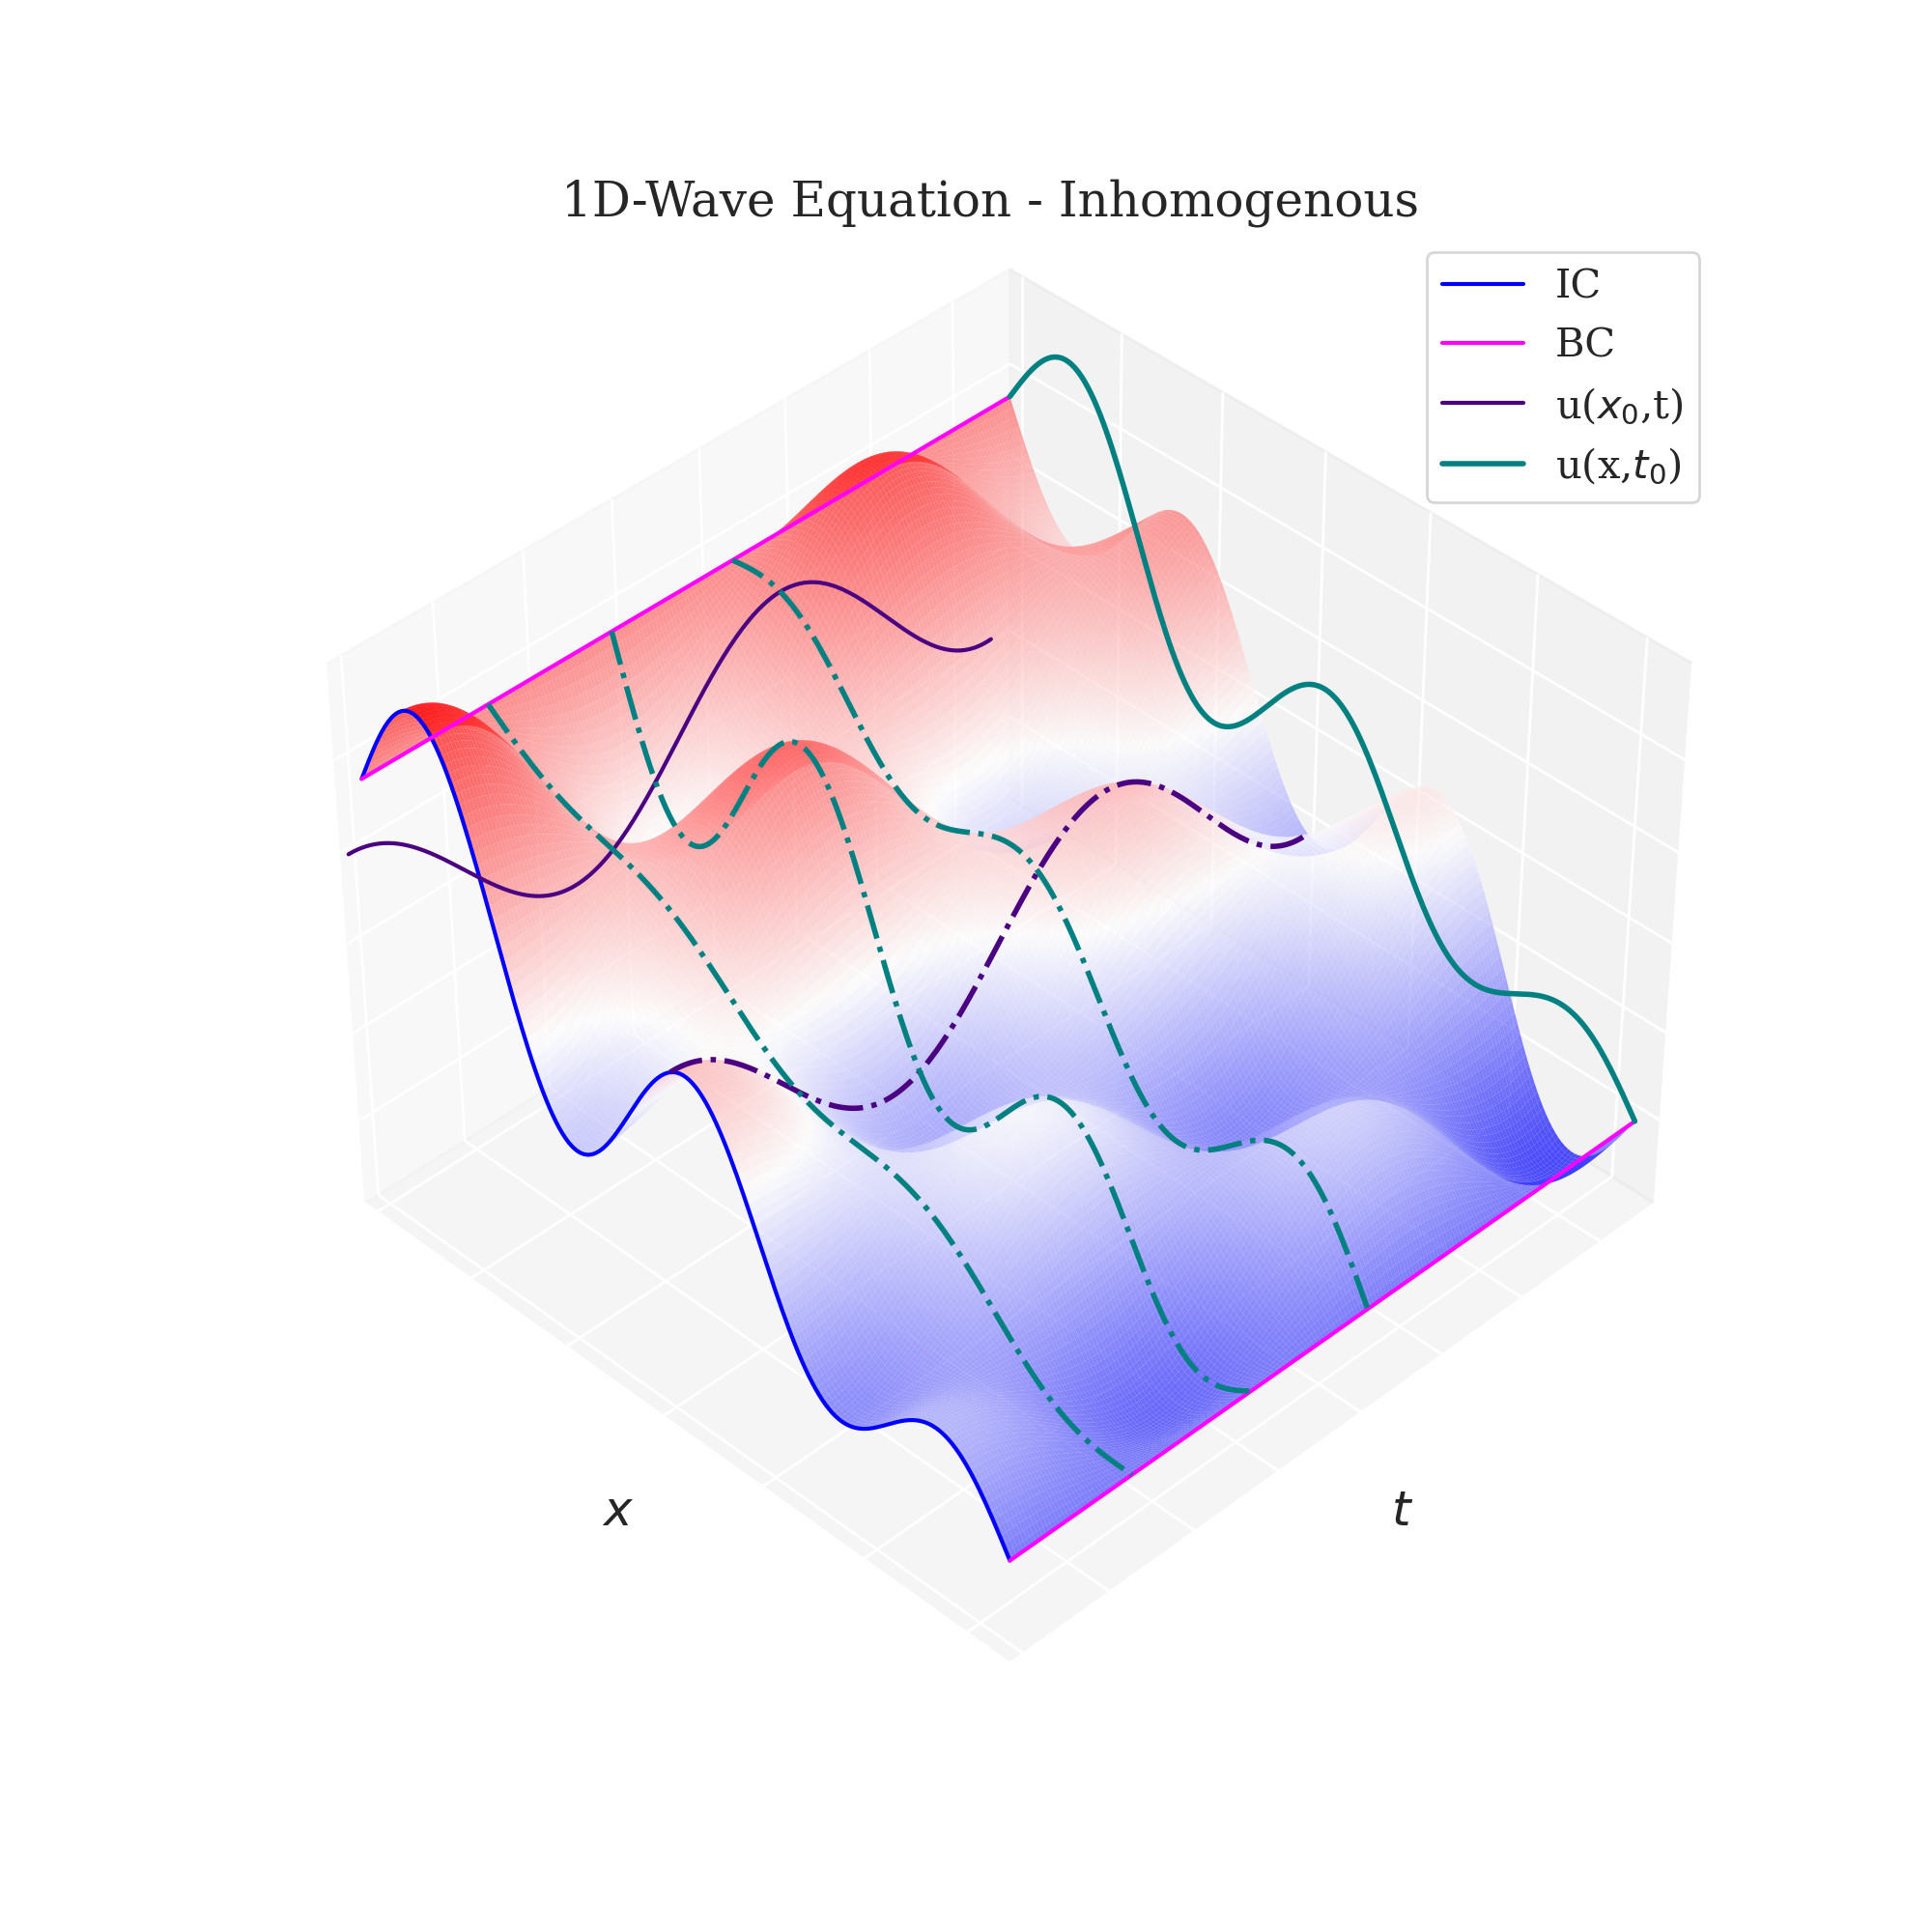
\includegraphics[width=0.85\linewidth]{../images/1d_wave_inhom.png}

\includegraphics[width=0.85\linewidth]{../images/1d_wave_fs.png}

\includegraphics[width=0.85\linewidth]{../images/1d_heat_fs.png}

\includegraphics[width=0.85\linewidth]{../images/2d_laplace.png}